\chapter{Experimental Study of Watershed Weighting Strategies}
\label{Chapter5}
\section{Evaluation}
\subsection{Dataset}
The Berkeley Segmentation Data Set (BSDS), introduced in~\cite{Martin01}, is a large dataset of natural images that have been manually segmented by multiple participants. It, therefore, provides the groundtruth label for each pixel as being on- or off-boundary. Initially the dataset featured 300 images (BSDS300). It was later extended - in BSDS500~\cite{Arbelaez11} the original 300 images are used for training (200) and validation (100), and 200 new human-annotated images are added for testing. Again, each image is segmented by different subjects.

\begin{figure}[ht!]
 \centering
 \subfigure[Input image]{%
 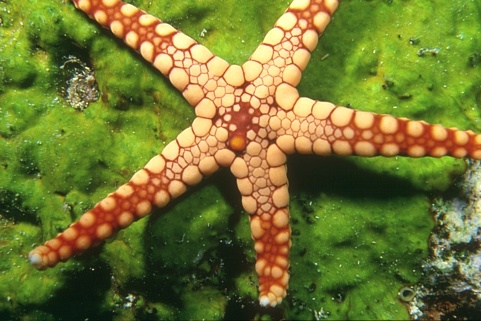
\includegraphics[width=0.3\textwidth]{images/examples/starfish/starfish.png}
 }
 \subfigure[Segmentation by subject 1]{%
 
\includegraphics[width=0.3\textwidth]{images/examples/starfish/starfish_segm_coarse.png}
 }
 \subfigure[Boundaries by subject 1]{%
 
\includegraphics[width=0.3\textwidth,frame]{images/examples/starfish/starfish_bdry_coarse.png}
 }
 \subfigure[Segmentation subject 2]{%
 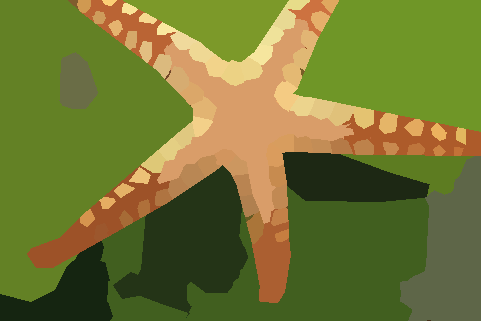
\includegraphics[width=0.3\textwidth]{images/examples/starfish/starfish_segm_detail.png}
 }
 \subfigure[Boundaries subject 2]{%
 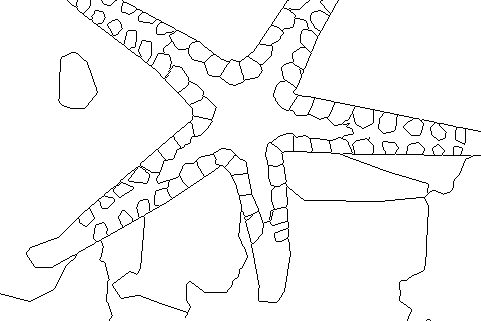
\includegraphics[width=0.3\textwidth,frame]{images/examples/starfish/starfish_bdry_detail.png}
 }
 \caption{Image from the validation subset of~\cite{BSDS500resources} and two of its annotations.}
\end{figure}

\subsection{Metrics}
\section{Exploration of the Space of Weighting Strategies}
\section{Oracle - Experiments with Ground Truth}
\subsection{Oracle Description}
\subsection{Ranking of Oracles}
\subsubsection{Confirms Correct Weighting Strategies}
\subsubsection{Failure Cases}
